\begin{appendices}
\appendix

\chapter{Example ScienceIE Training/Test Document}
\label{appendix:egpaper}
The following is ScienceIE test paper file S0010938X15301268.txt:\\

\noindent Fig. 9 displays the growth of two of the main corrosion products that develop or form on the surface of Cu40Zn with time, hydrozincite (Fig. 9a) and Cu2O (Fig. 9b). It should be remembered that both phases were present already from start of the exposure. The data is presented in absorbance units and allows comparisons to be made of the amounts of each species between the two Cu40Zn surfaces investigated, DP and HZ7. The tendency is very clear that the formation rates of both hydrozincite and cuprite are quite suppressed for Cu40Zn with preformed hydrozincite (HZ7) compared to the diamond polished surface (DP). In summary, without being able to consider the formation of simonkolleite, it can be concluded that an increased surface coverage of hydrozincite reduces the initial spreading ability of the NaCl-containing droplets and thereby lowers the overall formation rate of hydrozincite and cuprite.

\chapter{Example ScienceIE Training/Test Annotation Data}
\label{appendix:egann}
The following is ScienceIE test paper annotations file S0010938X15301268.ann:\\

\noindent T1	Material 46 64	corrosion products
T2	Material 104 110	Cu40Zn\\
T3	Material 122 134	hydrozincite\\
T4	Material 149 153	Cu2O\\
T5	Material 378 384	Cu40Zn\\
T6	Material 408 410	DP\\
T7	Material 415 418	HZ7\\
T8	Material 530 536	Cu40Zn\\
T9	Material 552 564	hydrozincite\\
T10	Material 566 569	HZ7\\
*	Synonym-of T9 T10\\
T11	Material 587 611	diamond polished surface\\
T12	Material 613 615	DP\\
*	Synonym-of T11 T12\\
T13	Material 678 691	simonkolleite\\
T14	Material 751 763	hydrozincite\\
T15	Material 809 833	NaCl-containing droplets\\
T16	Material 883 895	hydrozincite\\
T17	Material 900 907	cuprite\\
T18	Process 456 471	formation rates\\
T20	Process 280 296	absorbance units\\
T19	Task 308 406	comparisons to be made of the amounts of each species between the two Cu40Zn surfaces investigated\\
R1	Hyponym-of Arg1:T3 Arg2:T1\\
R2	Hyponym-of Arg1:T4 Arg2:T1\\
T21	Material 480 492	hydrozincite\\
T22	Material 497 504	cuprite\\
T23	Process 665 691	formation of simonkolleite\\
T24	Process 776 793	initial spreading\\
T25	Process 865 879	formation rate\\

\chapter{Stop Words List}
\label{appendix:stopwords}
Below is the list of stop words used in this project:\\
\begin{multicols}{7}
\noindent !!\\
?!\\
??\\
!?\\
`\\
``\\
''\\
-lrb-\\
-rrb-\\
-lsb-\\
-rsb-\\
,\\
.\\
:\\
;\\
"\\
'\\
?\\
$<$\\
$>$\\
\{\\
\}\\
$[$\\
$]$\\
+\\
-\\
(\\
)\\
\&\\
\%\\
\$\\
@\\
!\\
\^\\
\#\\
*\\
..\\
...\\
'll\\
's\\
'm\\
a\\
about\\
above\\
after\\
again\\
against\\
all\\
am\\
an\\
and\\
any\\
are\\
aren't\\
as\\
at\\
be\\
because\\
been\\
before\\
being\\
below\\
between\\
both\\
but\\
by\\
can\\
can't\\
cannot\\
could\\
couldn't\\
did\\
didn't\\
do\\
does\\
doesn't\\
doing\\
don't\\
down\\
during\\
each\\
few\\
for\\
from\\
further\\
had\\
hadn't\\
has\\
hasn't\\
have\\
haven't\\
having\\
he\\
he'd\\
he'll\\
he's\\
her\\
here\\
here's\\
hers\\
herself\\
him\\
himself\\
his\\
how\\
how's\\
i\\
i'd\\
i'llv
i'm\\
i've\\
if\\
in\\
into\\
is\\
isn't\\
it\\
it's\\
its\\
itself\\
let's\\
me\\
more\\
most\\
mustn't\\
my\\
myself\\
no\\
nor\\
not\\
of\\
off\\
on\\
once\\
only\\
or\\
other\\
ought\\
our\\
ours\\
ourselves\\
out\\
over\\
own\\
same\\
shan't\\
she\\
she'd\\
she'll\\
she's\\
should\\
shouldn't\\
so\\
some\\
such\\
than\\
that\\
that's\\
the\\
their\\
theirs\\
them\\
themselves\\
then\\
there\\
there's\\
these\\
they\\
they'd\\
they'll\\
they're\\
they've\\
this\\
those\\
through\\
to\\
too\\
under\\
until\\
up\\
very\\
was\\
wasn't\\
we\\
we'd\\
we'll\\
we're\\
we've\\
were\\
weren't\\
what\\
what's\\
when\\
when's\\
where\\
where's\\
which\\
while\\
who\\
who's\\
whom\\
why\\
why's\\
with\\
won't\\
would\\
wouldn't\\
you\\
you'd\\
you'll\\
you're\\
you've\\
your\\
yours\\
yourself\\
yourselves\\
\#\#\#\\
return\\
arent\\
cant\\
couldnt\\
didnt\\
doesnt\\
dont\\
hadnt\\
hasnt\\
havent\\
hes\\
heres\\
hows\\
im\\
isnt\\
its\\
lets\\
mustnt\\
shant\\
shes\\
shouldnt\\
thats\\
theres\\
theyll\\
theyre\\
theyve\\
wasnt\\
were\\
werent\\
whats\\
whens\\
wheres\\
whos\\
whys\\
wont\\
wouldnt\\
youd\\
youll\\
youre\\
youve\\
\end{multicols}

\chapter{Google Scholar and ScienceDirect Search Pages}
\label{appendix:searcheg}
The following are screen shots of the query "computer science" being queried in two popular search engines: Google Scholar (left) and ScienceDirect (right). The "\textbf{$\cdot$$\cdot$$\cdot$}" denote some of the search results has been cropped out. As cropping has been applied, the results presented by Google Scholar and ScienceDirect are 10 and 25 (configurable to 50 or 100) respectively. \\

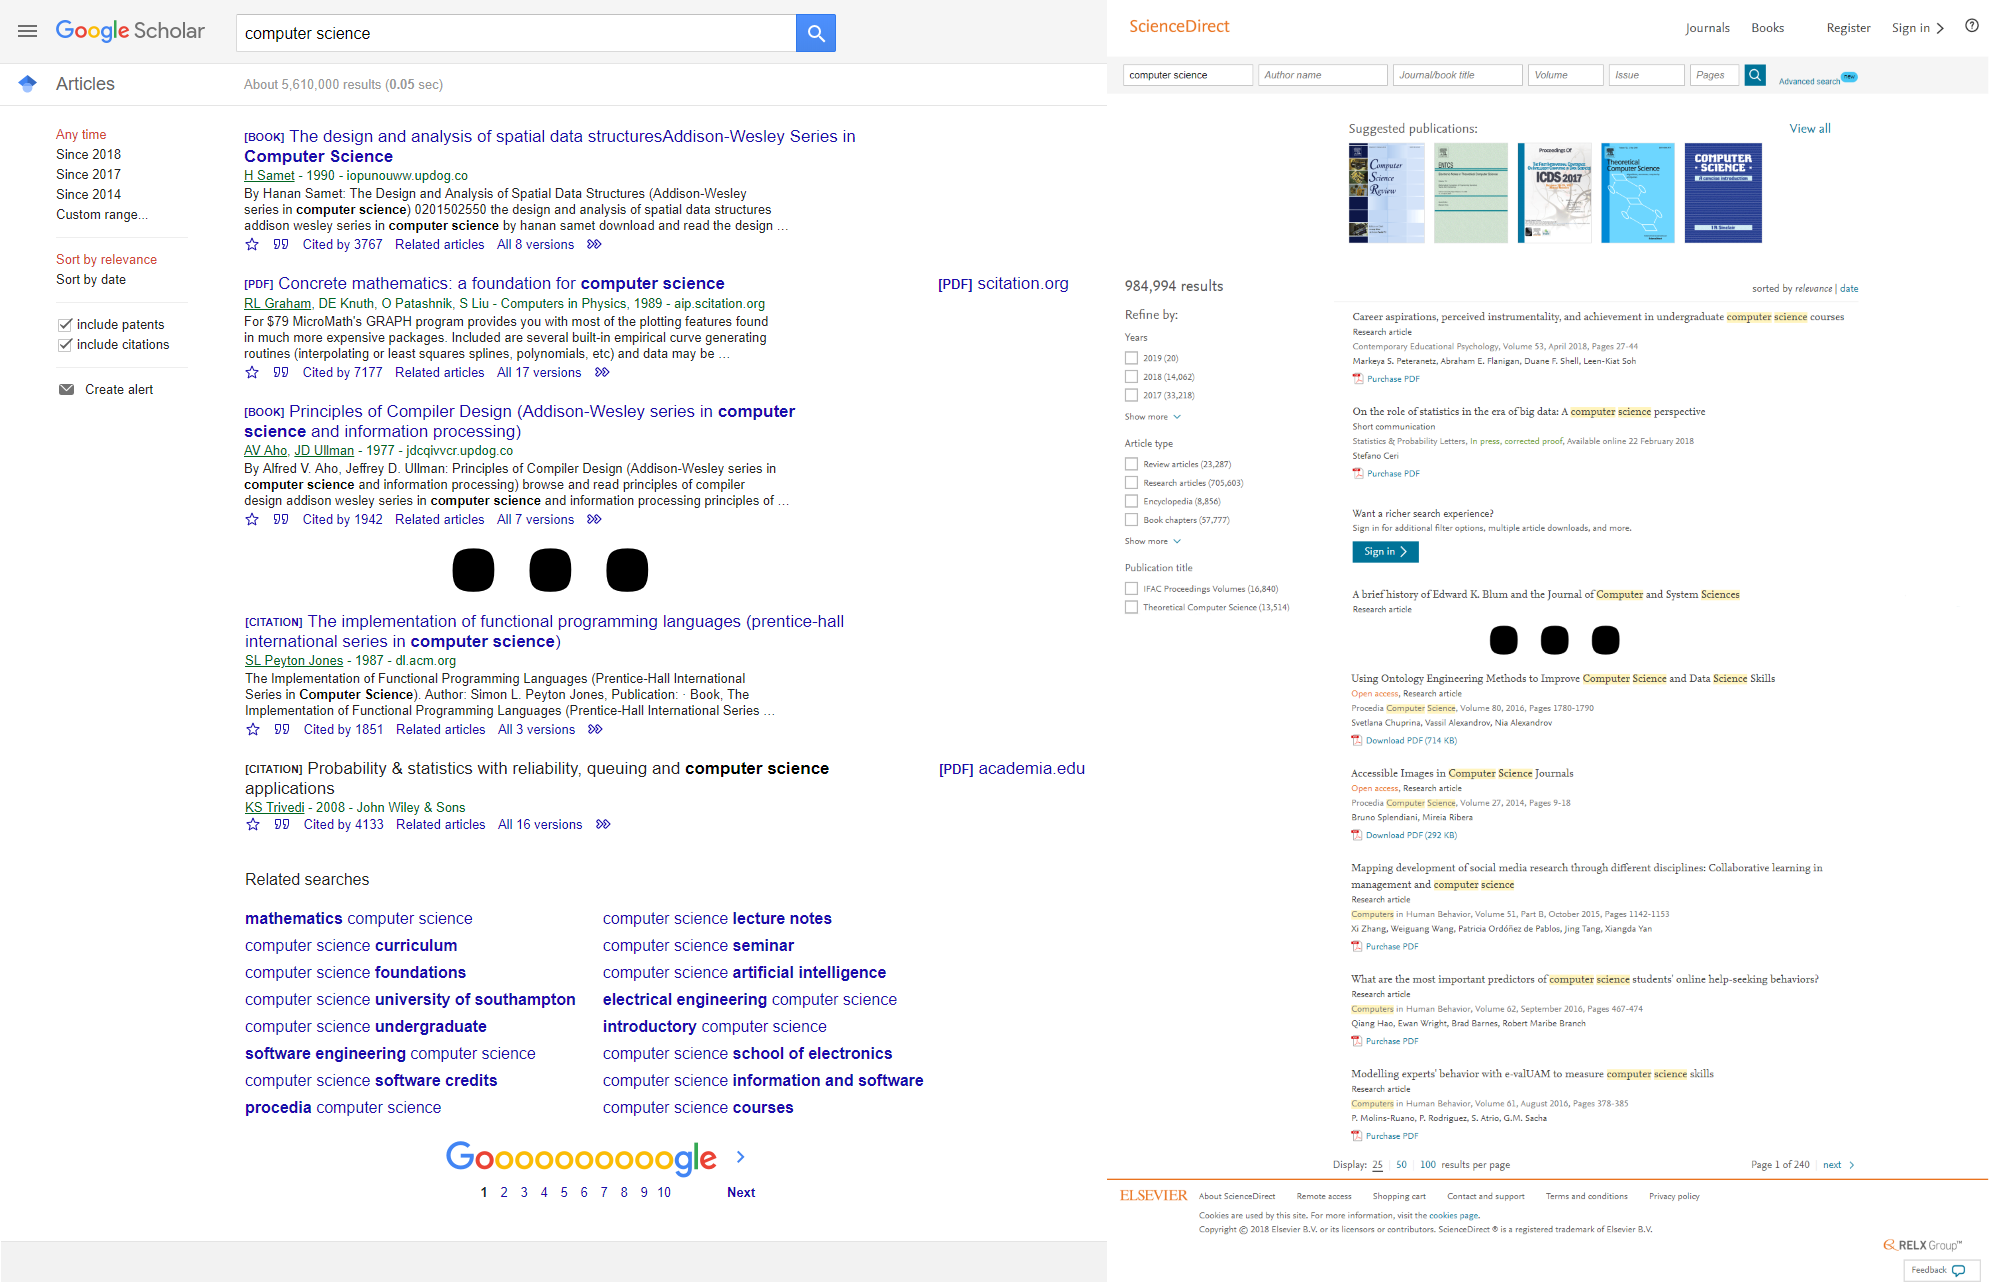
\includegraphics[width=\textwidth]{img/searchexamples.png}

\chapter{How to run the project from source}
\label{appendix:howtorun}

To run the two applications, the following prerequisite steps must be taken:
\begin{enumerate}
	\item Install Java 8, Maven 3 and MySQL.
	\begin{itemize}
		\item Running \texttt{./install\_*.sh} in \texttt{resources/scripts} will do this for a system with \texttt{apt-get} available, such as Ubuntu.
	\end{itemize}
	\item Run the \texttt{env\_maven\_opts.sh} script in \texttt{resources/scripts} to setup required system environment variables.
	\item A Word2Vec model is needed. Based on this report, the pre-trained Google News model\footnote{\href{https://drive.google.com/file/d/0B7XkCwpI5KDYNlNUTTlSS21pQmM/}{https://drive.google.com/file/d/0B7XkCwpI5KDYNlNUTTlSS21pQmM/}} is recommended for download.
\end{enumerate}

\noindent Some files required by the system need pointing to. 
In terms of training and testing paper locations, checking the \texttt{paper.txt} and \texttt{test\_papers.txt} in the resource folders of both Java projects should reveal the paths used on the development system. The paths listed in this file are all processed unless they begin with a \texttt{\#}, and either point to a text file for processing, or a directory containing multiple text files for processing. Change these appropriately. 

Other components are more embedded in the Java code. Ideally a better solution to this should have been included by the developer, but unfortunately other tasks used up this time. Change \texttt{log4j2.xml:8} and \texttt{NlpObjectStore.java:23} to any folder where logs and serialised files can be saved. Change \texttt{Word2VecPretrained.java:11} to point to a Word2Vec model (either the Google News model or a model renamed to the same file descriptor).

To setup the MySQL database, navigate to \texttt{resources/sql}. Run, in order, \texttt{./setup.sh} and \texttt{./build.sh}. If you wish to use the final data made in this project run \texttt{./recover.sh}. Depending upon your MySQL configuration, you may need to change the password to be stronger. Finally, update \texttt{application.properties} in the FYP-GUI project's resource folder with the correct connection string and password.

Navigate to the root of the two Java projects (both in \texttt{java/}), and a series of useful scripts for compiling and running are presented: \\

\noindent \begin{tabular}{ l | p{3.5cm} | p{9cm} }
	\textbf{Java Project} & \textbf{Script} & \textbf{Description} \\
	\hline
	FYP-NLP & \texttt{./build.sh} & Compiles the system, without running any tests. \\
	\hline
	FYP-NLP & \texttt{./install.sh} & Compiles the system, without running any tests, and installs the project to the local Maven repository (required for building the FYP-GUI project). \\
	\hline
	FYP-NLP & \texttt{./test.sh $<$test class$>$} & Compiles the system and runs the JUnit test class given. Test classes can be found in \texttt{java/FYP-NLP/src/test/java/xyz/tomclarke/fyp/nlp}, and specifying the name of the class will run all test methods inside it without \texttt{@Ignore} above the \texttt{@Test} annotation.  \\
	\hline
	FYP-GUI & \texttt{./build.sh} & Compiles the GUI and runs all JUnit tests. \\
	\hline
	FYP-GUI & \texttt{./build-and-run.sh} & Compiles the GUI, without running any tests, and launches the GUI. \\
	\hline
	FYP-GUI & \texttt{./run.sh} & Launches the GUI (assumes it is already built). \\
\end{tabular}

\end{appendices}
